\section{MDD example}
\label{sec:mdd_example}
In this section we provide an example of a \mdd\ reduction for the language $\mathcal{L} = \{\omega \in \{0, 1\}^4 \mid \omega[2] = 1\}$, that are all the binary of length $4$ with a $1$ in the second position as a constraint. In \cref{fig:mmd1} we have the full \mdd\ representation, and we can immediately see that the red branches can be ignored since they do not respect the constraint. After their elimination (\cref{fig:mmd2}), we see that the nodes $19$ and $20$ have same father and are both accepting states. Therefore, they are compatible and apt to be merged (a same reasoning case be made on the pairs of nodes $21$ and $22$, $28$ and $29$, $30$ and $31$ with their respectively fathers). In $\cref{fig:mmd3}$, we see that the two sub-paths going from state $4$ to \textit{tt} can be merged: they both lead to the accepting state and their suffix is identical w.r.t the labels on their edges. We continue this way until the reduction operation in no more feasible in order to obtain the final \mdd\ depicted in \cref{fig:mmd5}.

\begin{figure}[!htb]
	\centering
	\begin{subfigure}[b]{1\linewidth}
		\centering
		\scalebox{.8}{
			\centering
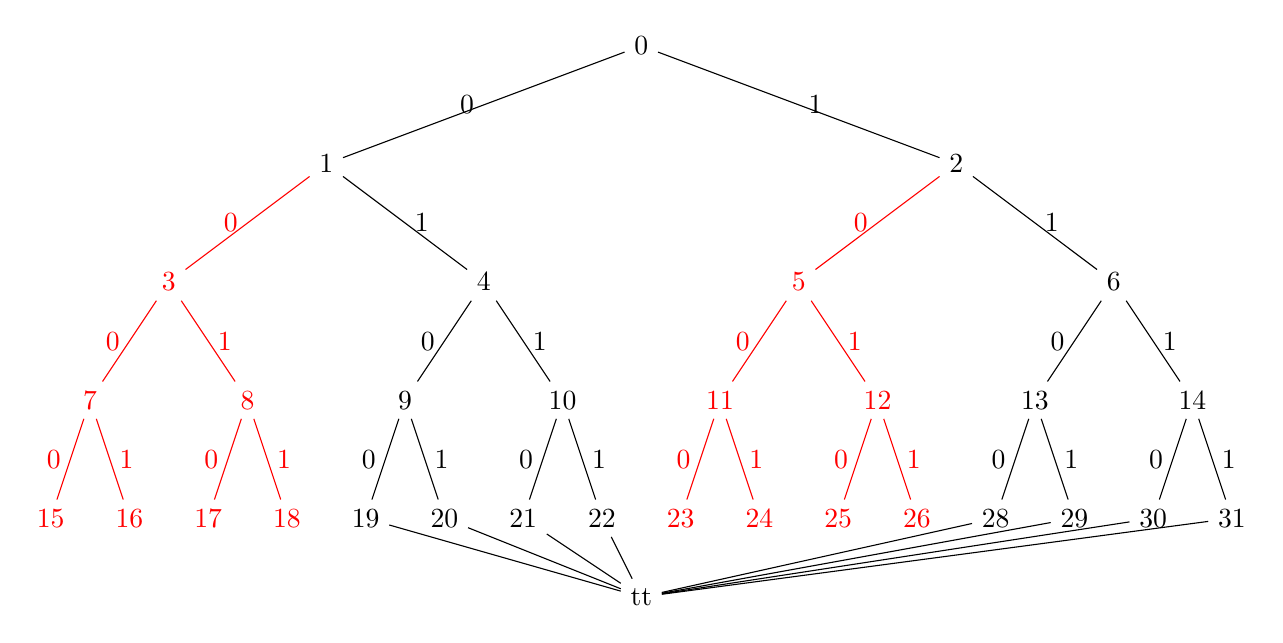
\begin{tikzpicture}
  [
    level 1/.style = {sibling distance = 8cm},
    level 2/.style = {sibling distance = 4cm},
    level 3/.style = {sibling distance = 2cm},
    level 4/.style = {sibling distance = 1cm},
  ]

  \node (root) at (0,0) {0}
  child {node {1}
      child [red] {
          node {3}
          child {node {7}
              child {node {15}
                  edge from parent node [left] {0}}
              child {node {16}
                  edge from parent node [right] {1}}
              edge from parent node [left] {0}}
          child {node {8}
              child {node {17}
                  edge from parent node [left] {0}}
              child {node {18}
                  edge from parent node [right] {1}}
              edge from parent node [right] {1}}
          edge from parent node [left] {0}}
      child {
          node {4}
          child {node {9}
              child {node {19}
                  edge from parent node [left] {0}}
              child {node {20}
                  edge from parent node [right] {1}}
              edge from parent node [left] {0}}
          child {node {10}
              child {node {21}
                  edge from parent node [left] {0}}
              child {node {22}
                  edge from parent node [right] {1}}
              edge from parent node [right] {1}}
          edge from parent node [right] {1}}
      edge from parent node [left] {0}
    }
  child {node {2}
      child [red] {
          node {5}
          child {node {11}
              child {node {23}
                  edge from parent node [left] {0}}
              child {node {24}
                  edge from parent node [right] {1}}
              edge from parent node [left] {0}}
          child {node {12}
              child {node {25}
                  edge from parent node [left] {0}}
              child {node {26}
                  edge from parent node [right] {1}}
              edge from parent node [right] {1}}
          edge from parent node [left] {0}}
      child {node {6}
          child {node {13}
              child {node {28}
                  edge from parent node [left] {0}}
              child {node {29}
                  edge from parent node [right] {1}}
              edge from parent node [left] {0}}
          child {node {14}
              child {node {30}
                  edge from parent node [left] {0}}
              child {node {31}
                  edge from parent node [right] {1}}
              edge from parent node [right] {1}}
          edge from parent node [right] {1}}
      edge from parent node [right] {1}
    };

  \node (bottomnode) at (0,-7) {tt};

  \foreach \w in {1,2}{
      \foreach \x in {1,2} {
          \foreach \y in {1, 2}{
              \draw (root-\w-2-\x-\y) -- (bottomnode);
            }
        }
    }

\end{tikzpicture}
		}
		\caption{Complete \mdd}
		\label{fig:mmd1}
	\end{subfigure}
\end{figure}

\begin{figure}[!htb]\ContinuedFloat
	\def\scale{.65}
	\centering
	\begin{subfigure}[b]{.34\linewidth}
		\centering
		\scalebox{\scale}{
			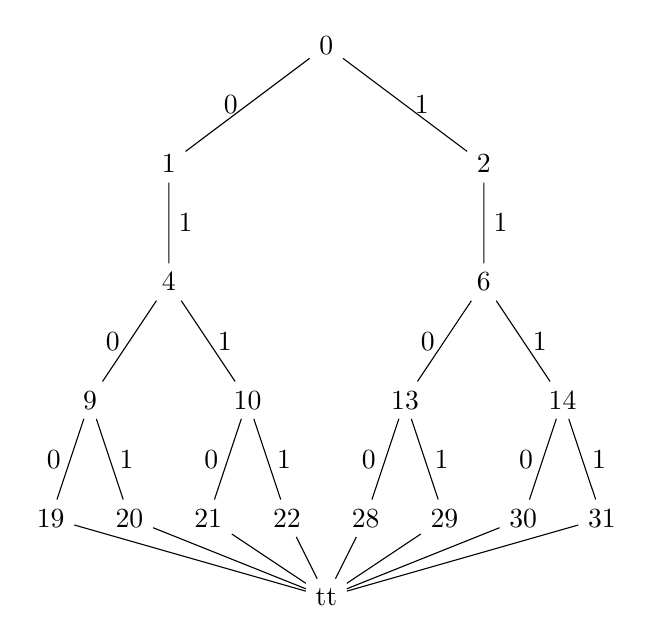
\begin{tikzpicture}
  [
    level 1/.style = {sibling distance = 4cm},
    level 2/.style = {sibling distance = 4cm},
    level 3/.style = {sibling distance = 2cm},
    level 4/.style = {sibling distance = 1cm},
  ]

  \node (root) at (0,0) {0}
  child {node {1}
      child {
          node {4}
          child {node {9}
              child {node {19}
                  edge from parent node [left] {0}}
              child {node {20}
                  edge from parent node [right] {1}}
              edge from parent node [left] {0}}
          child {node {10}
              child {node {21}
                  edge from parent node [left] {0}}
              child {node {22}
                  edge from parent node [right] {1}}
              edge from parent node [right] {1}}
          edge from parent node [right] {1}}
      edge from parent node [left] {0}
    }
  child {node {2}
      child {node {6}
          child {node {13}
              child {node {28}
                  edge from parent node [left] {0}}
              child {node {29}
                  edge from parent node [right] {1}}
              edge from parent node [left] {0}}
          child {node {14}
              child {node {30}
                  edge from parent node [left] {0}}
              child {node {31}
                  edge from parent node [right] {1}}
              edge from parent node [right] {1}}
          edge from parent node [right] {1}}
      edge from parent node [right] {1}
    };

  \node (bottomnode) at (0,-7) {tt};

  \foreach \w in {1,2}{
      \foreach \x in {1,2} {
          \foreach \y in {1, 2}{
              \draw (root-\w-1-\x-\y) -- (bottomnode);
            }
        }
    }

\end{tikzpicture}
		}
		\caption{Deletion of dead branches}
		\label{fig:mmd2}
	\end{subfigure}
	\hfill
	\begin{subfigure}[b]{.34\linewidth}
		\centering
		\scalebox{\scale}{
			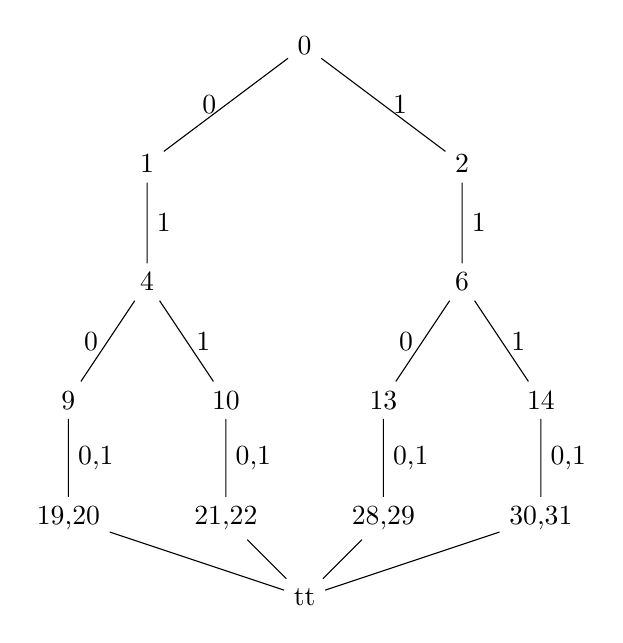
\begin{tikzpicture}
  [
    level 1/.style = {sibling distance = 4cm},
    level 2/.style = {sibling distance = 2cm},
    level 4/.style = {sibling distance = 1cm},
  ]

  \node (root) at (0,0) {0}
  child {node {1}
      child {
          node {4}
          child {node {9}
              child {node {19,20}
                  edge from parent node [right] {0,1}}
              edge from parent node [left] {0}}
          child {node {10}
              child {node {21,22}
                  edge from parent node [right] {0,1}}
              edge from parent node [right] {1}}
          edge from parent node [right] {1}}
      edge from parent node [left] {0}
    }
  child {node {2}
      child {node {6}
          child {node {13}
              child {node {28,29}
                  edge from parent node [right] {0,1}}
              edge from parent node [left] {0}}
          child {node {14}
              child {node {30,31}
                  edge from parent node [right] {0,1}}
              edge from parent node [right] {1}}
          edge from parent node [right] {1}}
      edge from parent node [right] {1}
    };

  \node (bottomnode) at (0,-7) {tt};

  \foreach \w in {1,2}{
      \foreach \x in {1,2} {
          \draw (root-\w-1-\x-1) -- (bottomnode);
        }
    }

\end{tikzpicture}
		}
		\caption{Reduction $1$}
		\label{fig:mmd3}
	\end{subfigure}
	\hfil
	\begin{subfigure}[b]{.15\linewidth}
		\centering
		\scalebox{\scale}{
			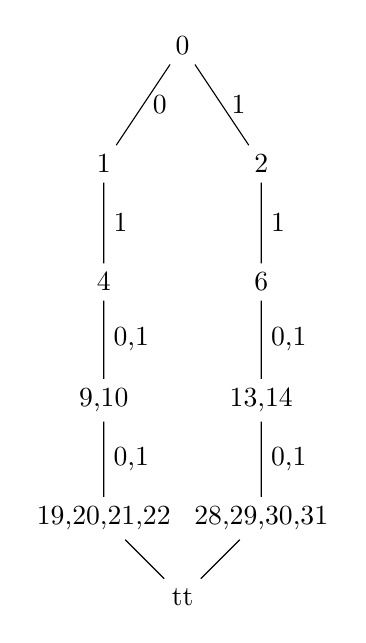
\begin{tikzpicture}
    [
        level 1/.style = {sibling distance = 2cm},
    ]

    \node (root) at (0,0) {0}
    child {node {1}
            child {
                    node {4}
                    child {node {9,10}
                            child {node {19,20,21,22}
                                    edge from parent node [right] {0,1}}
                            edge from parent node [right] {0,1}}
                    edge from parent node [right] {1}}
            edge from parent node [right] {0}
        }
    child {node {2}
            child {node {6}
                    child {node {13,14}
                            child {node {28,29,30,31}
                                    edge from parent node [right] {0,1}}
                            edge from parent node [right] {0,1}}
                    edge from parent node [right] {1}}
            edge from parent node [right] {1}
        };

    \node (bottomnode) at (0,-7) {tt};

    \foreach \w in {1,2}{
            \draw (root-\w-1-1-1) -- (bottomnode);
        }

\end{tikzpicture}
		}
		\caption{Reduction $2$}
		\label{fig:mmd4}
	\end{subfigure}
	\hfill
	\begin{subfigure}[b]{.15\linewidth}
		\centering
		\scalebox{\scale}{
			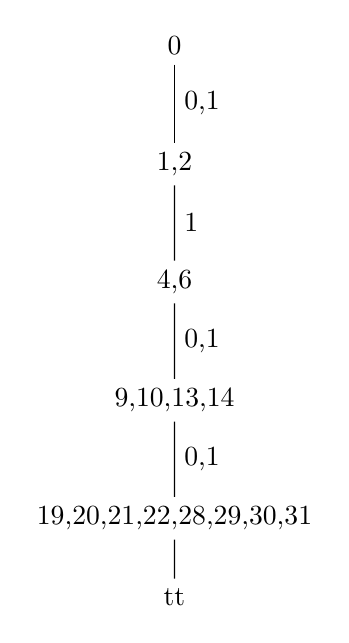
\begin{tikzpicture}

  \node (root) at (0,0) {0}
  child {node {1,2}
      child {
          node {4,6}
          child {node {9,10,13,14}
              child {node {19,20,21,22,28,29,30,31}
                  edge from parent node [right] {0,1}}
              edge from parent node [right] {0,1}}
          edge from parent node [right] {1}}
      edge from parent node [right] {0,1}
    };

  \node (bottomnode) at (0,-7) {tt};

  \draw (root-1-1-1-1) -- (bottomnode);

\end{tikzpicture}
		}
		\caption{Reduction $3$}
		\label{fig:mmd5}
	\end{subfigure}

	\caption{\mdd\ for $\mathcal{L}$}
	\label{fig:mmd}
\end{figure}